\section*{Introduction}

\begin{frame}{\tt ./whoami}
  \begin{columns}
    \column{.65\textwidth}
    \textbf{Léo Lavaur}
    \begin{itemize}
      \item Postdoctoral research fellow at SnT, University of Luxembourg since Dec. 2024.
      \item PhD in Computer Science from IMT Atlantique (2024). \textit{Best PhD Thesis Award} from the GDR RSD\footnotemark[1] in 2025.
      \item Engineering degree from ENSIBS, 2020.
      \item Industry experience: 4 years in work-study programs, inc. 3 at Orange Cyberdefense.
    \end{itemize}

    \medskip\small
    Keywords: intrusion detection, federated/decentralized machine learning, logic programming, neural-symbolic learning, cybersecurity datasets.

    \column{.35\textwidth}
    \centering
    \includegraphics[width=.8\linewidth]{figures/lavaur_snt.png} 
  \end{columns}

  \footnotetext[1]{CNRS's research group on networks and distributed systems.}
\end{frame}

% \begin{frame}{Information Security}
%   \begin{figure}
%     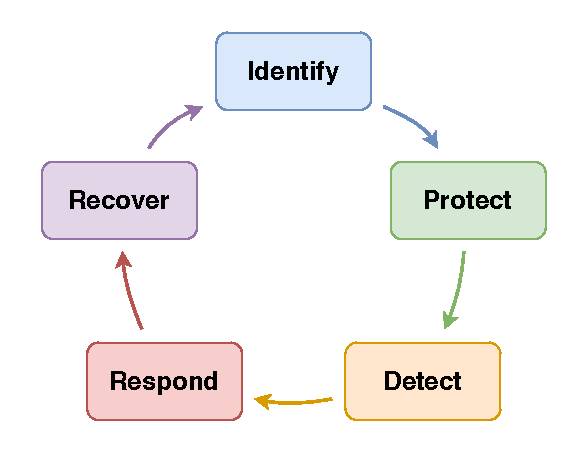
\includegraphics[width=.4\linewidth]{figures/thesis/intro/security.drawio.pdf}
%     \caption*{The security life-cycle \footcite{nationalinstituteofstandardsandtechnology_NISTCybersecurityFramework_2024}.}
%   \end{figure}
% \end{frame}

% \begin{frame}{The Need for Collaboration}
%   \centering
%   \foreach \i in {1,...,4} {%
%     \includegraphics<\i>[width=.9\textwidth]{figures/thesis/intro/collab/collab-\i.drawio.pdf}%
%   }
% \end{frame}

\begin{frame}{Machine Learning for Intrusion Detection}
  % \begin{columns}
  %   \begin{column}{.6\textwidth}
  %     \sntoptions{block=fill}
  %     \begin{block}{Intrusion Detection System (IDS)}
  %       \medskip
  %       IDSs monitor the behavior of a system to detect malicious activities.
  %     \end{block}
  %   %   \begin{itemize}
  %   %     \item Collaboration pushed by:
  %   %     \begin{itemize}[<+->]
  %   %       \item common interest (\eg, inter-SOCs\footnotemark);
  %   %       \item national agencies (\eg, NIST, ENISA, ANSSI);
  %   %       \item regulation (\eg, private-public information sharing in NIS2).
  %   %     \end{itemize}
  %   %   \end{itemize}
  %   \end{column}
  \begin{columns}
    \column{.4\textwidth}
    \centering
    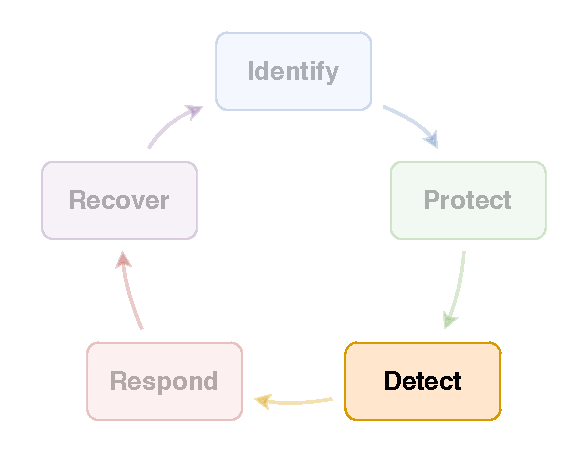
\includegraphics[width=\linewidth]{figures/thesis/intro/security-focus.drawio.pdf}
  
    \column{.6\textwidth}
    \textbf{Solved problem?}
    \begin{itemize}[<+->]
      \item Deep Learning (DL) offers very high performance\dots{} \onslide<+->\emph{on public datasets at least}.
      \item Various strategies: \alert<+->{supervised}, unsupervised, semi-supervised, reinforcement learning, \etc.
    \end{itemize}
  \end{columns}

\end{frame}




\begin{frame}{IDS Deployment Challenges}
  % \stepcounter{beamerpauses}
  % \bigskip
  % \only<+>{}%
  % \begin{itemize}[<+->]
  %   \item Over-representation of Deep Learning, offering high performance (DL)\dots{} \onslide<+->\emph{on public datasets at least}.
  %   \item Various strategies: \alert<+->{supervised}, unsupervised, semi-supervised, reinforcement learning, \etc.
  % \end{itemize}
    % \item Great performance with Deep Learning (DL)\dots{}
    % \onslide<+->
    % \emph{on public datasets at least}.
  % \end{itemize}
  % \bigskip
  
  \onslide<+->
  \begin{columns}
    \begin{column}{0.5\textwidth}
      %\bigskip
      \begin{block}{Challenges of local training}
        \begin{itemize}
          \item not enough labelled data;
          \item risk of local bias or skewed data distribution.
          % \item inefficient against new attacks, especially \alert{supervised} approaches.
        \end{itemize}
      \end{block}
      \onslide<+->{
      \begin{block}{Push for collaboration}
        \begin{itemize}
          \item common interest (\eg, inter-SOCs\footnotemark);
          \item national agencies (\eg, NIST, ANSSI);
          \item regulation (\eg, private-public information sharing in NIS2).
        \end{itemize}
      \end{block}
      }
    \end{column}
    \onslide<1->
    \begin{column}{0.5\textwidth}
      \begin{figure}
        \centering
        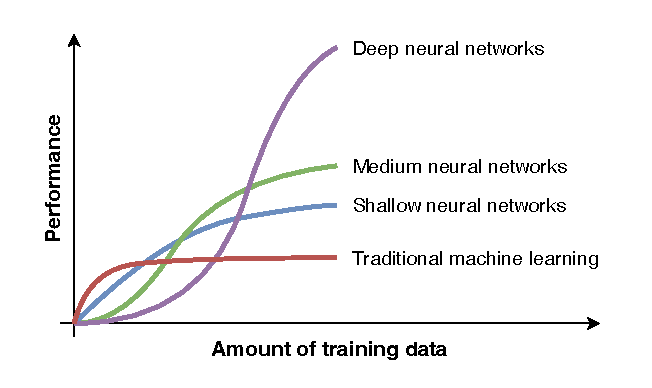
\includegraphics[width=\linewidth]{figures/thesis/intro/ml-perf}
      \end{figure}
    \end{column}
  \end{columns}
\end{frame}

\begin{frame}{Data Sharing to the Rescue?}
% TODO:
% pas assez de données, faisons un pot commun !
% oui mais non :
% - confidentialité des données 
% - confiance dans le point de collecte
% - confiance dnas le processus d'apprentissage
% - pas de modèle de detection sans serveur
\begin{columns}
  \begin{column}{0.5\textwidth}
    \centering
    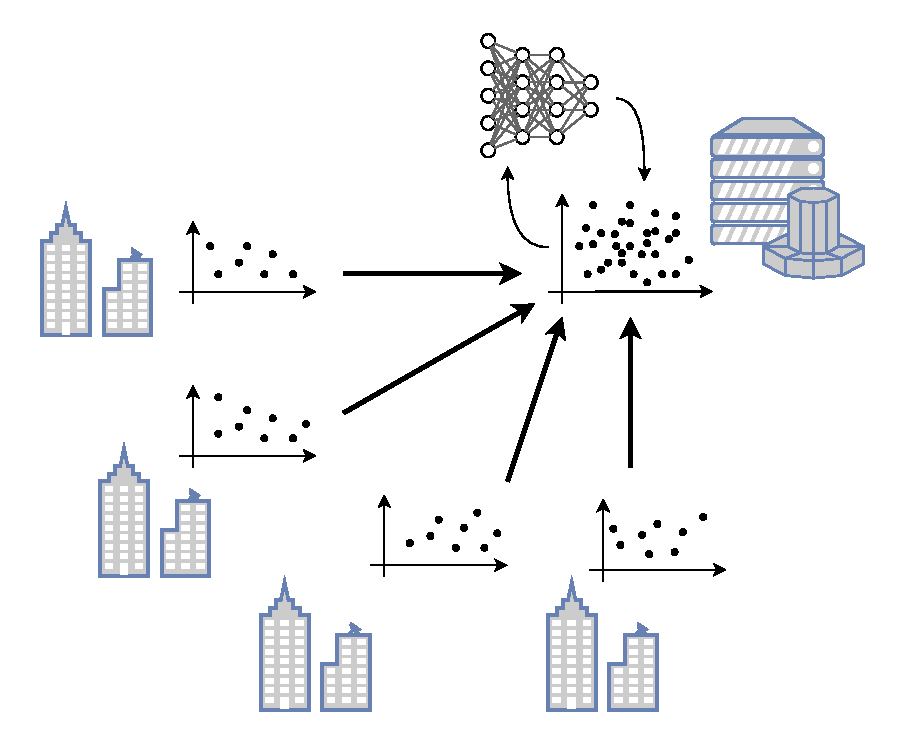
\includegraphics[width=\linewidth]{figures/thesis/intro/collab.pdf}
  \end{column}
  \begin{column}{0.5\textwidth}
    \textbf{Let's pool our data!}\pause{} \textbf{Although\dots}
    \begin{itemize}
      \item Privacy concerns.
      \item Lack of trust in the data holder.
      \item Lack of trust in the learning process.
      %\item Lack of incentives.
      \item \dots
    \end{itemize}
  \end{column}
\end{columns}
\end{frame}

\begin{frame}{Scaling Intrusion Detection}
  \begin{columns}
    \column{.45\textwidth}
    \begin{block}{Federated Learning (FL)}
      \begin{itemize}
        \item Recent-\textit{ish} distributed ML paradigm~\autocite{mcmahan_Communicationefficientlearningdeep_2017}.
        \item Clients train a common model without sharing their training data.
        \item \alert{Privacy-preserving}: model sharing partially prevents data leakage.
      \end{itemize}
    \end{block}

    \column{.55\textwidth}
    \begin{figure}
      \centering
      % \foreach \i in {1,...,7} {%
      %   \includegraphics<\i>[width=\linewidth]{./figures/thesis/intro/fl/\i.pdf}%
      % }
      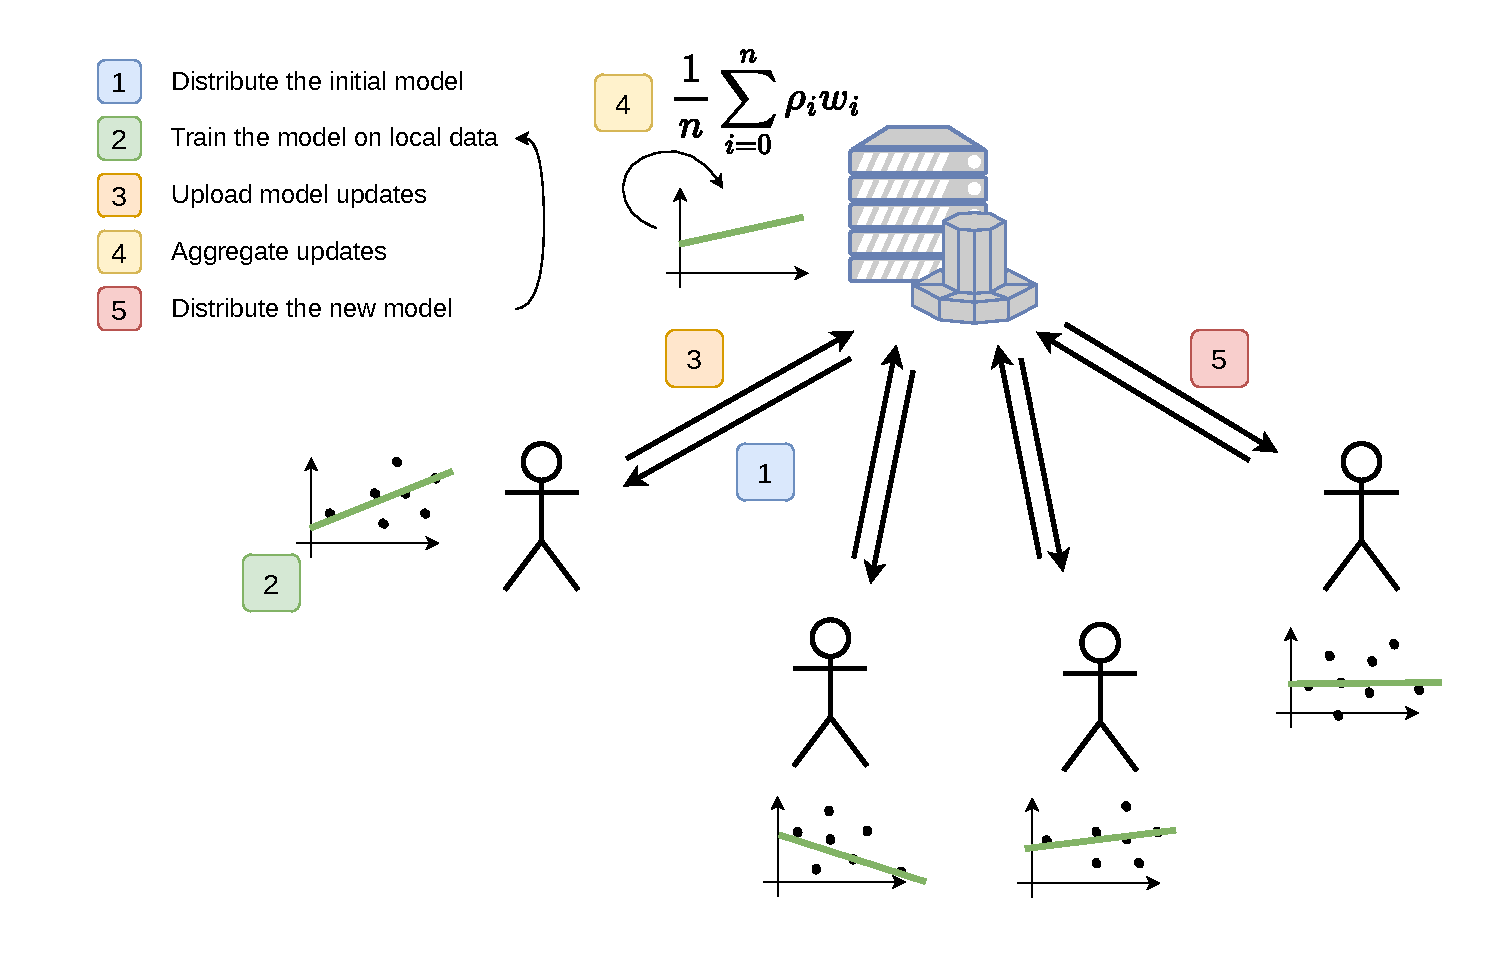
\includegraphics[width=\linewidth]{./figures/feditn/intro/fl.drawio.pdf}
      \caption{Typical FL workflow}
  \end{figure}
  \end{columns}

  \footcite*{mcmahan_Communicationefficientlearningdeep_2017}
\end{frame}


% \begin{frame}{FL Fundamentals}
%   \begin{figure}
%     \centering
%     \foreach \i in {1,...,7} {%
%       \includegraphics<\i>[width=.75\linewidth]{./figures/thesis/intro/fl/\i.pdf}%
%     }
%     \caption{Typical FL workflow, applied to NIDSs.}
%   \end{figure}
% \end{frame}

